\documentclass{article}
\usepackage{titlesec}
\usepackage[page]{totalcount}
\usepackage{graphicx}
\author{Chang Liu}
\title{Caffe: Convoluational Architecture for Fast Feature Embedding}


\begin{document}

\newpagestyle{main}{
	\sethead{Chang Liu}{Caffe Notes}{chang\_liu\\@student.uml.edu}
	\setfoot{}{}{\thepage \// \totalpages}
	\headrule
	\footrule
}

\pagestyle{main}

\maketitle

\tableofcontents
\newpage


\section{Abstract}

This section gives a basic idea about Caffe, which is as follows that matter:

1) C++ libarary with Python and Matlab binding for training and deploying

2) General convolutional neural network and \textbf{other deep-learning models}

3) CUDA GPU computing, with 40 million images a day on single K40 or Titan GPU


\section{Introduction}

Selction:

1) hand-craft feature is not as good as learning features in representing images.

2) It usually takes months to replicate the result of others' research, which makes it hard for improving.

3) By designing Caffe, it gives a very good result and application in research and industry.

\begin{center}
%includegraphics[width=4.00in, height=2.00in]{Caffe_Note_1.png}
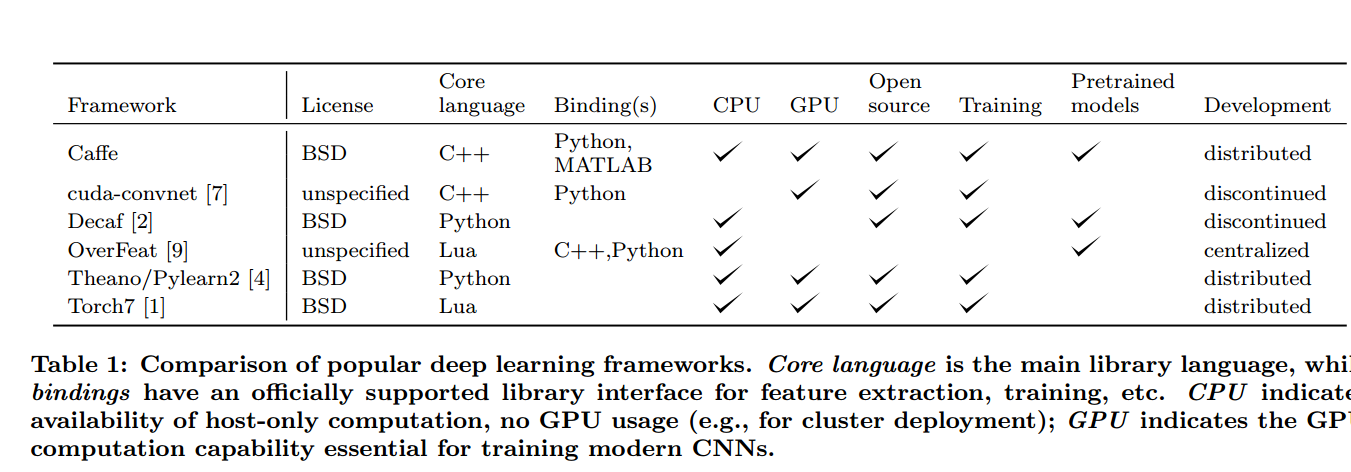
\includegraphics[scale=0.25]{Caffe_Note_1.png}
\end{center}


\section{Highlights}

these advantages:

1) Modularity. easy extension to new data.

2) Separation of representation and implementation. model defintion using Proftocol BUffer.

3) Test coverage.

4) Python and MATLAB binding.

5) Pre-trained reference models. AlexNet, ImageNet, R-CNN models


\subsection{Comparing to other software}
These contributions make the Caffe outstanding to other software:

1) Caffe is purely C++ based, making it easy to integration to existing C++ system.

2) Reference model is provided for quick experiment, without need for costly re-learning.


\section{Architecture}

This section gives a very good description about Caffe's structure.

\subsection{Data storage}

Main points:

1). communicates data in 4-dimensional array called blobs.

2). conceal the computational and mental overhead of mixed CPU/GPU.

3). Large scale data is store in LevelDB database, layer-wise design...


\subsection{Layers}

A couple of layers types, includes, convolution,
pooling, inner products, nonlinearities like rectified
linear and logistic, local response normalization, elementwise
operations, and losses like softmax and hinge 


\subsection{Network and Run Mode}

CPU/GPU mixture.

\subsection{Training A network}

reduces the loss and gradients which train the whole network. This example is found in the Caffe source code at examples\//lenet\//lenet\_train.prototxt. Data are processed in mini-batches that pass through the network sequentially. Vital to training are learning rate decay schedules, momentum, and snapshots for stopping and resuming, all of which are implemented and documented.

\begin{center}
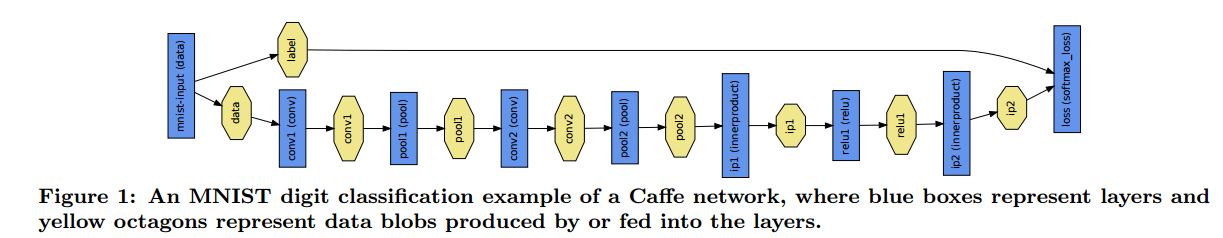
\includegraphics[scale=0.25]{Caffe_Note_2.png}
\end{center}



\subsection{Application and Examples}
\subsection{Object Classification}
models: 10,000 categories of the full ImageNet dataset by finetuning
this network

\subsection{Learning Semantic Features}





\subsection{Object Detection}
Girshick et al. have combined Caffe together with techniques
such as Selective Search to effectively perform
simultaneous localization and recognition in natural images


\end{document}


